\documentclass[conference]{IEEEtran}
\IEEEoverridecommandlockouts
% The preceding line is only needed to identify funding in the first footnote. If that is unneeded, please comment it out.
\usepackage{cite}
\usepackage{amsmath,amssymb,amsfonts}
\usepackage{algorithmic}
\usepackage{graphicx}
\usepackage{textcomp}
\usepackage{xcolor}
\usepackage{float}
\usepackage{tikz}
\usepackage{listofitems} % for \readlist to create arrays
\usetikzlibrary{arrows.meta} % for arrow size
% STYLES
\tikzset{
  >=latex, % for default LaTeX arrow head
  node/.style={thick,circle,draw=myblue,minimum size=22,inner sep=0.5,outer sep=0.6},
  node in/.style={node,green!20!black,draw=mygreen!30!black,fill=mygreen!25},
  node hidden/.style={node,blue!20!black,draw=myblue!30!black,fill=myblue!20},
  node convol/.style={node,orange!20!black,draw=myorange!30!black,fill=myorange!20},
  node out/.style={node,red!20!black,draw=myred!30!black,fill=myred!20},
  connect/.style={thick,mydarkblue}, %,line cap=round
  connect arrow/.style={-{Latex[length=4,width=3.5]},thick,mydarkblue,shorten <=0.5,shorten >=1},
  node 1/.style={node in}, % node styles, numbered for easy mapping with \nstyle
  node 2/.style={node hidden},
  node 3/.style={node out}
}
\def\nstyle{int(\lay<\Nnodlen?min(2,\lay):3)} % map layer number onto 1, 2, or 3

\usepackage[outline]{contour} % glow around text
\contourlength{1.4pt}

\tikzset{>=latex} % for LaTeX arrow head

% COLORS
\usepackage{xcolor}
\colorlet{myred}{red!80!black}
\colorlet{myblue}{blue!80!black}
\colorlet{mygreen}{green!60!black}
\colorlet{myorange}{orange!70!red!60!black}
\colorlet{mydarkred}{red!30!black}
\colorlet{mydarkblue}{blue!40!black}
\colorlet{mydarkgreen}{green!30!black}
\usetikzlibrary{shapes, arrows, positioning}
\def\BibTeX{{\rm B\kern-.05em{\sc i\kern-.025em b}\kern-.08em
    T\kern-.1667em\lower.7ex\hbox{E}\kern-.125emX}}
\begin{document}

\title{Autonomous closed-loop guidance using reinforcement learning in a low-thrust, multi-body dynamical environment*\\
{\footnotesize \textsuperscript{*}Reinforcement Learning Course Project Report}
\thanks{Identify applicable funding agency here. If none, delete this.}
}

\author{\IEEEauthorblockN{Ali Baniasad}
\IEEEauthorblockA{\textit{Department of Aerospace Engineering} \\
\textit{Sharif University of Technology}\\
Tehran, Iran \\
ali\_baniasad@ae.sharif.edu}
\and
\IEEEauthorblockN{Mehrdad Boroushaki}
\IEEEauthorblockA{\textit{Department of Energy Engineering} \\
\textit{Sharif University of Technology}\\
Tehran, Iran \\
boroushaki@sharif.edu}
}

\maketitle

\begin{abstract}
    Onboard autonomy is an essential component in enabling increasingly complex missions into deep space. In nonlinear dynamical environments, computationally efficient guidance strategies are challenging. Many traditional approaches rely on either simplifying assumptions in the dynamical model or on abundant computational resources. This research effort employs reinforcement learning, a subset of machine learning, to produce a 'lightweight' closed-loop controller that is potentially suitable for onboard low-thrust guidance in challenging dynamical regions of space. The results demonstrate the controller's ability to directly guide a spacecraft despite large initial deviations and to augment a traditional targeting guidance approach. The proposed controller functions without direct knowledge of the dynamical model; direct interaction with the nonlinear equations of motion creates a flexible learning scheme that is not limited to a single force model, mission scenario, or spacecraft. The learning process leverages high-performance computing to train a closed- loop neural network controller. This controller may be employed onboard to autonomously generate low-thrust control profiles in real-time without imposing a heavy workload on a flight computer. Control feasibility is demonstrated through sample transfers between Lyapunov orbits in the Earth-Moon system. The sample low- thrust controller exhibits remarkable robustness to perturbations and generalizes effectively to nearby motion. Finally, the flexibility of the learning framework is demonstrated across a range of mission scenarios and low-thrust engine types.
\end{abstract}

\begin{IEEEkeywords}
    Reinforcement learning-based, computationally efficient closed-loop control enables autonomous low-thrust guidance in complex deep-space missions, showcasing flexibility across diverse scenarios without relying on explicit dynamical models.
\end{IEEEkeywords}

\section{Introduction}
Advancements in onboard autonomy are enabling new opportuni- ties for establishing a sustained human and robotic presence in deep space. In complex multi-body dynamical environments, such as in the Earth–Moon neighborhood, onboard applications for low-thrust spacecraft are particularly challenging. This investigation demonstrates Reinforcement Learning (RL), a subset of Machine Learning (ML), to be an effective approach for automated closed-loop guidance in these challenging regions of space. Onboard autonomous guidance requires a computationally efficient approach that addresses nonlinearity in the dynamical model and offers flexibility as requirements change inflight. In satisfying these criteria, RL provides a model-agnostic approach for training a neural network controller that is applicable to multiple problems, and potentially suitable for onboard use.
\section{Problem formulation}
The three-body problem serves as a suitable dynamical model that is representative of observed natural motion in cislunar space. While the proposed guidance framework does not depend on any particular model, the planar Circular Restricted Three-Body Problem (CR3BP) serves as a useful environment for preliminary evaluation because it both represents a challenging region of space that is relevant to upcoming missions while sufficiently low-fidelity for initial analysis of the guidance scheme. Additionally, low-thrust propulsion is included to demonstrate algorithmic performance despite limited control authority and pronounced nonlinearities. While the proposed guidance scheme directly supplies a control history, an alternative concept of operations leverages the trained neural network to produce an initial guess for other numerical methods, such as targeting or optimization schemes. A sample direct multiple shooting algorithm is included in this analysis to demonstrate the added value of the neural network to the onboard targeting capability.

\subsection{Dynamical model}

The CR3BP is a model for the motion of an infinitesimal mass moving under the influence of two celestial bodies. In this model, two spherically symmetric gravitational bodies, \(P_1\) and \(P_2\) form the primary system as they move in circular orbits about their common barycenter, B; \(P_3\) moves freely with respect to the barycenter. The motion of \(P_3\) is governed by the following equations of motion:
\begin{equation}
    \ddot{x} - 2\dot{y} = \frac{\partial U}{\partial x} + u\frac{\partial U}{\partial \dot{x}}
\end{equation}
\begin{equation}
    \ddot{y} + 2\dot{x} = \frac{\partial U}{\partial y} + u\frac{\partial U}{\partial \dot{y}}
\end{equation}
where \(U\) is the effective potential function and \(u\) is the dimensionless thrust parameter. The effective potential function is defined as:
\begin{equation}
    U = \frac{1}{2}(x^2 + y^2) + \frac{1 - \mu}{r_1} + \frac{\mu}{r_2}
\end{equation}

\section{Guidance framework design}
\subsection{Reinforcement learning overview}
Reinforcement Learning (RL) is a branch of machine learning that encompasses a broad range of goal-oriented algorithms that 'learn' to perform tasks by means of trial-and-error. Current state-of-the-art RL approaches employ modern advancements in neural networks to aid in challenging tasks. Policy gradient methods are of particular recent interest due to their demonstrated ability in continuous control tasks. One such algorithm, Proximal Policy Optimization (PPO), is employed in this investigation to train a neural network controller.
\subsubsection{Neural Network}
A Neural Network (NN) is a class of nonlinear statistical models that are frequently employed in ML classification and regression tasks [44]. The term neural network encompasses many different types of statistical models with various levels of complexity. When applied correctly, NNs perform exceedingly well, and are a driving factor in ML advancements over the past decade. While frequently used in supervised learning applications, NNs are also employed extensively in modern RL algorithms due to their demonstrated ability in approximating nonlinear functions. Many traditional tabular RL approaches, such as Q-learning, rely on finely discretizing the state and action spaces, quickly becoming impractical as the number of dimensions in the problem increases. Leveraging NNs allows modern algorithms to both access continuous state and action spaces and to easily incorporate additional dimensions.
Evaluating a feedforward neural network consists of straightforward linear algebra operations, with several nonlinear element-wise activation functions. After the input layer, each node is computed as a linear combination of weighted values and a bias, and processed through an activation function to incorporate nonlinearity into the model [44]. The weights signify the impact that particular nodes exert on each node in the next layer. The bias allows the activation function to be shifted left or right for each node. Together, the weights and biases form the set of trainable parameters for the model. In general, these parameters cannot be known a-priori, and so no suitable initial guess for their value is possible. Hence, the weights in this investigation are randomly initialized according to a normal distribution of zero mean and the biases are initialized to zero.
Without activation functions, the network is only able to model linear functions and, thus, the selection of the activation function is an important component in neural network performance. Furthermore, bounded functions are advantageous since they aid in normalizing the output of each neuron. This investigation employs hyperbolic tangent (\(\tanh\)) to bound outputs and incorporate nonlinearity. Linear activation is also, at times, advantageous. Within RL, networks that produce a single scalar output value frequently employ a linear activation in the output layer. Together, \(\tanh\) and linear are the only two activation functions employed in this investigation, with \(\tanh\) used in all hidden layers and linear used in the output layer.
%% add tanh figure
\begin{figure}[H]
    \centering
    \includegraphics[width=0.5\textwidth]{../Figures/Hyperbolic_Tangent.png}
    \caption{Hyperbolic tangent activation function}
\label{fig:tanh}
\end{figure}

\subsubsection{Reinforcement learning fundamentals}
Reinforcement learning is a class of algorithms in which a goal- seeking agent seeks to complete a task by means of interaction with an environment. An agent is a controller that maps observed variables to actions. The learning process originates with the agent directly exploring an environment by means of trial-and-error. The environment communicates relevant information about its dynamics to the agent by means of a state signal, which the agent then employs to perform some action. The environment updates its current state based on the action and computes a numerical reward that communicates the immediate benefit of the given action. This process repeats iteratively such that, over time, the agent improves its policy (the means by which decisions are accomplished) by seeking to maximize the reward signal. In many cases, terminal conditions exist that cause the learning process to cease. In these cases, the environment typically resets to an initial configuration, and the process begins anew. These are identified as episodic tasks, where each episode signifies an attempt by the agent to solve a problem. A schematic for the high-level process of an RL agent is depicted in Fig~\ref{fig:agent-env}. This diagram highlights the three signals that enable communication between the agent and environment at time steps \(t\) and \(t+1\): state, action, and reward. While the RL literature prefers the terms agent, environment, and action, these expressions are analogous to the more common engineering terms controller, controlled system (or plant), and control signal.
\begin{figure}[H]
    \centering
    \includegraphics[width=0.5\textwidth]{../Figures/agent-env.png}
    \caption{Reinforcement learning agent-environment interaction}
    \label{fig:agent-env}
\end{figure}

Without external supervision, the agent uncovers complex dynam- ical structures that inform decision-making. This procedure is char- acterized as a Markov Decision Process (MDP), which involves both feedback and associative actions, and are a classical formalization of sequential decision-making problems. The MDP is the idealized mathematical form of the problem, and allows for theoretical analysis of the RL process. In the infinite-horizon discounted case, the MDP is formulated by a tuple \((S, A, P, R, \gamma)\), where \(S\) is the set of possible states, \(A\) is the set of possible actions, \(P\) is the transition probability function, \(R\) is the reward function, and \(\gamma\) is the discount factor. The transition probability function is defined as \(P(s_{t+1}|s_t, a_t)\), which is the probability of transitioning to state \(s_{t+1}\) given that the agent is in state \(s_t\) and performs action \(a_t\). The reward function is defined as \(R(s_t, a_t)\), which is the reward received by the agent for performing action \(a_t\) in state \(s_t\). The discount factor is a scalar value in the range \([0, 1]\) that determines the relative importance of future rewards. The goal of the agent is to maximize the expected discounted return, \(G_t\), which is defined as:
\begin{equation}
    G_t = \sum_{k=0}^{\infty}\gamma^kR_{t+k+1}
\end{equation}
where \(R_{t+k+1}\) is the reward received at time \(t+k+1\). The discount factor is used to ensure that the sum converges. The agent's policy, \(\pi\), is a mapping from states to actions, and is defined as:
\begin{equation}
    \pi(a|s) = P(a_t = a|s_t = s)
\end{equation}
where \(\pi(a|s)\) is the probability of performing action \(a\) in state \(s\). The goal of the agent is to maximize the expected return by selecting the optimal policy, \(\pi^*\), which is defined as:
\begin{equation}
    \pi^* = \arg\max_{\pi}E[G_t|s_t, \pi]
\end{equation}
where \(E[G_t|s_t, \pi]\) is the expected return given that the agent is in state \(s_t\) and follows policy \(\pi\). The optimal policy is the policy that maximizes the expected return for all states. The optimal value function, \(V^*\), is defined as:
\begin{equation}
    V^*(s) = \max_{\pi}E[G_t|s_t = s, \pi]
\end{equation}
where \(V^*(s)\) is the expected return given that the agent is in state \(s\) and follows the optimal policy. The optimal action-value function, \(Q^*\), is defined as:
\begin{equation}
    Q^*(s, a) = \max_{\pi}E[G_t|s_t = s, a_t = a, \pi]
\end{equation}
where \(Q^*(s, a)\) is the expected return given that the agent is in state \(s\), performs action \(a\), and follows the optimal policy. The optimal value function and optimal action-value function are related as:
\begin{equation}
    V^*(s) = \max_{a}Q^*(s, a)
\end{equation}
\begin{equation}
    Q^*(s, a) = R(s, a) + \gamma\sum_{s'}P(s'|s, a)V^*(s')
\end{equation}

\section{Policy Gradient Methods}

Policy Gradient Methods are a class of reinforcement learning algorithms that directly optimize the policy of an agent in order to maximize the expected cumulative reward. Unlike value-based methods, which estimate the value function and then derive a policy from it, policy gradient methods directly parameterize the policy and update its parameters to improve performance.

\subsection{Objective Function}

The goal of policy gradient methods is to find a policy $\pi_{\theta}$ parameterized by $\theta$ that maximizes the expected cumulative reward:

\begin{equation}
J(\theta) = \mathbb{E}_{\tau \sim \pi_{\theta}} \left[ \sum_{t=0}^{\infty} \gamma^t r_t \right],
\end{equation}

where $\tau$ represents a trajectory, $r_t$ is the reward at time step $t$, and $\gamma$ is the discount factor.

\subsection{Policy Parameterization}

The policy is often parameterized as a probability distribution over actions given the state, i.e., $\pi_{\theta}(a|s)$. Common parameterizations include softmax functions applied to action preferences or directly using neural networks.

\subsection{Policy Gradient Theorem}

The key insight in policy gradient methods is the Policy Gradient Theorem, which provides a gradient expression for the expected cumulative reward with respect to the policy parameters:

\begin{equation}
\nabla_{\theta} J(\theta) \propto \mathbb{E}_{\tau \sim \pi_{\theta}} \left[ \sum_{t=0}^{\infty} \nabla_{\theta} \log \pi_{\theta}(a_t|s_t) \cdot \left( \sum_{t'=t}^{\infty} \gamma^{t'-t} r_{t'} \right) \right].
\end{equation}

This gradient is then used to update the policy parameters in the direction that increases the expected cumulative reward.

\subsection{REINFORCE Algorithm}

One of the simplest policy gradient algorithms is the REINFORCE algorithm. It approximates the gradient using sampled trajectories and updates the policy parameters through stochastic gradient ascent.

\subsection{Actor-Critic Methods}

To reduce variance and improve sample efficiency, actor-critic methods combine policy gradient updates with value function estimates. The actor (policy) is updated using the advantage function, which measures how much better or worse an action is compared to the expected value.

\subsection{Advantages and Challenges}

Policy gradient methods have advantages, such as the ability to handle continuous action spaces and directly optimize non-differentiable policies. However, they often suffer from high variance, requiring careful design and hyperparameter tuning.

In summary, policy gradient methods provide a powerful framework for training agents in reinforcement learning settings by directly optimizing policies to maximize cumulative rewards.

\section{Deep Deterministic Policy Gradients (DDPG)}

Deep Deterministic Policy Gradients (DDPG) is a model-free, off-policy reinforcement learning algorithm that combines the strengths of both deep neural networks and deterministic policies. DDPG is particularly well-suited for problems with continuous action spaces, commonly encountered in robotic control and other real-world applications.

\subsection{Actor-Critic Architecture}

DDPG utilizes an actor-critic architecture, consisting of both an actor network and a critic network. The actor network parameterizes the policy, producing continuous actions, while the critic network evaluates the quality of the actions taken by the actor.

The actor network is denoted by $\mu(s|\theta^{\mu})$, where $\theta^{\mu}$ are the actor network parameters. The critic network is denoted by $Q(s, a|\theta^{Q})$, where $\theta^{Q}$ are the critic network parameters.

\subsection{Deterministic Policy Gradient}

DDPG employs the deterministic policy gradient to update the actor network. The objective function to be maximized is given by:

\begin{equation}
J(\theta^{\mu}) = \mathbb{E}_{s_t \sim \rho^{\beta}, a_t \sim \mu(s_t|\theta^{\mu}), s_{t+1} \sim P} \left[ Q(s_t, a_t|\theta^{Q}) \right],
\end{equation}

where $\rho^{\beta}$ is a replay buffer distribution and $P$ is the environment transition dynamics.

The deterministic policy gradient is then computed as:

\begin{equation}
\nabla_{\theta^{\mu}} J \approx \mathbb{E}_{s_t \sim \rho^{\beta}} \left[ \nabla_{a} Q(s, a|\theta^{Q}) |_{s=s_t, a=\mu(s_t)} \nabla_{\theta^{\mu}} \mu(s|\theta^{\mu}) |_{s=s_t} \right].
\end{equation}

\subsection{Experience Replay}

To improve stability and sample efficiency, DDPG employs an experience replay buffer. This buffer stores past experiences $(s_t, a_t, r_t, s_{t+1})$ and samples mini-batches for training both the actor and critic networks.

\subsection{Target Networks}

To stabilize the training process, DDPG introduces target networks for both the actor and critic. Target networks are slowly updated versions of the original networks, and this helps prevent the learning process from being overly influenced by the most recent experiences.

\subsection{Algorithm Summary}

The DDPG algorithm can be summarized as follows:

\begin{enumerate}
  \item Initialize actor and critic networks, target networks, and replay buffer.
  \item Sample a mini-batch from the replay buffer.
  \item Compute target values for the critic using target networks.
  \item Update critic by minimizing the temporal difference error.
  \item Update actor using the deterministic policy gradient.
  \item Update target networks slowly towards the current networks.
  \item Repeat steps 2-6 until convergence.
\end{enumerate}

\subsection{Advantages and Considerations}

DDPG has shown success in solving a variety of continuous control tasks. However, proper tuning of hyperparameters is crucial for its performance. Additionally, DDPG might face challenges in handling tasks with high-dimensional action spaces or sparse rewards.

In summary, DDPG is a powerful algorithm for continuous control problems, combining the benefits of deep neural networks and deterministic policies.

\section{Soft Actor-Critic (SAC)}

Soft Actor-Critic (SAC) is a state-of-the-art off-policy reinforcement learning algorithm designed for continuous action spaces. SAC addresses the challenges of sample efficiency and stability in deep reinforcement learning, and it belongs to the family of actor-critic algorithms.

\subsection{Entropy Regularized Policy Optimization}

SAC introduces entropy regularization to the policy optimization objective. The objective function is a combination of expected cumulative reward and entropy, defined as:

\begin{equation}
J(\theta) = \mathbb{E}_{\tau \sim \pi_{\theta}} \left[ \sum_{t=0}^{\infty} \gamma^t \left( r_t + \alpha H(\pi_{\theta}(\cdot|s_t)) \right) \right],
\end{equation}

where $\pi_{\theta}$ is the policy, $H(\pi_{\theta})$ is the entropy of the policy, and $\alpha$ is the temperature parameter controlling the trade-off between reward maximization and entropy maximization.

\subsection{Actor-Critic Architecture}

Similar to DDPG, SAC uses an actor-critic architecture. The actor network parameterizes the policy, and the critic network evaluates the quality of the actions. The objective for the actor is the entropy-regularized expected return:

\begin{equation}
J_{\text{actor}}(\theta) = \mathbb{E}_{a_t \sim \pi_{\theta}(\cdot|s_t)} \left[ Q_{\phi}(s_t, a_t) - \alpha \log \pi_{\theta}(a_t|s_t) \right],
\end{equation}

where $Q_{\phi}$ is the critic network and $\phi$ are its parameters.

\subsection{Entropy Regularization}

The entropy term in the objective function encourages exploration by penalizing overly deterministic policies. The overall objective encourages the policy to explore more diverse actions, leading to better generalization and robustness.

\subsection{Critic Update}

The critic is trained to minimize the Bellman residual:

\begin{align}
&J_{\text{critic}}(\phi) =\\ &\mathbb{E}_{(s_t, a_t, r_t, s_{t+1}) \sim \mathcal{D}} \left[ \frac{1}{2} \left( Q_{\phi}(s_t, a_t) - (r_t + \gamma V_{\text{target}}(s_{t+1})) \right)^2 \right],
\end{align}

where $V_{\text{target}}$ is the target value function.

\subsection{Temperature Update}

The temperature parameter $\alpha$ is updated to balance exploration and exploitation:

\begin{equation}
\alpha \leftarrow \alpha - \eta \cdot \nabla_{\alpha} \left( \mathbb{E}_{a_t \sim \pi_{\theta}(\cdot|s_t)} \left[ \alpha \log \pi_{\theta}(a_t|s_t) - \alpha \right] \right),
\end{equation}

where $\eta$ is the learning rate for the temperature parameter.

\subsection{Algorithm Summary}

The SAC algorithm can be summarized as follows:

\begin{enumerate}
  \item Initialize actor, critic, and target networks.
  \item Initialize temperature parameter $\alpha$.
  \item Collect samples from the environment.
  \item Update critic parameters using the Bellman residual.
  \item Update actor parameters using the entropy-regularized objective.
  \item Update temperature parameter using the gradient of the entropy term.
  \item Update target networks slowly towards the current networks.
  \item Repeat steps 3-7 until convergence.
\end{enumerate}

\subsection{Advantages and Considerations}

SAC has demonstrated strong performance in a variety of continuous control tasks. Its entropy regularization encourages effective exploration, and the algorithm is known for its stability and sample efficiency. However, tuning the temperature parameter and other hyperparameters is crucial for optimal performance.

In summary, Soft Actor-Critic is a versatile algorithm that excels in handling continuous action spaces and offers a principled approach to balancing exploration and exploitation through entropy regularization.

\section{Twin Delayed DDPG (TD3)}

Twin Delayed DDPG (TD3) is an off-policy reinforcement learning algorithm that builds upon the Deep Deterministic Policy Gradients (DDPG) algorithm. TD3 introduces several enhancements to address issues such as overestimation bias and instability during training, leading to improved performance in continuous control tasks.

\subsection{Enhancements Over DDPG}

TD3 incorporates the following key enhancements over DDPG:

\begin{enumerate}
  \item \textbf{Twin Q-Networks:} TD3 uses two Q-networks to estimate the value function, and the minimum value among them is used to reduce overestimation bias. This is in contrast to DDPG, which uses a single Q-network.

  \item \textbf{Target Policy Smoothing:} To stabilize training, TD3 introduces target policy smoothing during the actor update. This involves adding noise to the target actions during the actor update, preventing the actor from exploiting small updates in the Q-values.

  \item \textbf{Delayed Policy Updates:} TD3 delays the update of the actor policy relative to the critic updates. This helps mitigate the issues arising from correlated updates and reduces the variance in the policy updates.

\end{enumerate}

\subsection{Actor-Critic Architecture}

Similar to DDPG, TD3 employs an actor-critic architecture. The actor network parameterizes the policy, and the critic network(s) evaluate the quality of the actions. The critic uses twin Q-networks, denoted as $Q_1$ and $Q_2$, to estimate the value function.

\subsection{Objective Function}

The objective function for the critic is given by:

\begin{align}
    &J_{\text{critic}}(\phi) =\\ &\mathbb{E}_{(s_t, a_t, r_t, s_{t+1}) \sim \mathcal{D}} \left[ \frac{1}{2} \left( Q_1(s_t, a_t) - y_t \right)^2 + \frac{1}{2} \left( Q_2(s_t, a_t) - y_t \right)^2 \right]
\end{align}
    

where $y_t = r_t + \gamma \min(Q_1'(s_{t+1}, a_t), Q_2'(s_{t+1}, a_t))$ is the target value.

The actor is updated to maximize:

\begin{equation}
J_{\text{actor}}(\theta^{\mu}) = -\mathbb{E}_{s_t \sim \rho^{\beta}} \left[ Q_1(s_t, \mu(s_t|\theta^{\mu})) \right],
\end{equation}

where $\rho^{\beta}$ is a replay buffer distribution.

\subsection{Target Network Updates}

The target networks $Q_1'$ and $Q_2'$ are updated slowly towards the current Q-networks:

\begin{equation}
\begin{split}
\theta^{Q'} &\leftarrow \rho \theta^Q + (1 - \rho) \theta^{Q'}, \\
\theta^{\mu'} &\leftarrow \rho \theta^{\mu} + (1 - \rho) \theta^{\mu'},
\end{split}
\end{equation}

where $\rho$ is the target network update coefficient.

\subsection{Algorithm Summary}

The TD3 algorithm can be summarized as follows:

\begin{enumerate}
  \item Initialize actor, twin Q-networks ($Q_1$ and $Q_2$), target networks ($Q_1'$ and $Q_2'$), and replay buffer.
  \item Sample a mini-batch from the replay buffer.
  \item Update twin Q-networks using the critic objective.
  \item Update actor using the actor objective.
  \item Update target networks slowly towards the current networks.
  \item Repeat steps 2-5 until convergence.
\end{enumerate}

\subsection{Advantages and Considerations}

TD3 addresses overestimation bias and instability during training, leading to improved sample efficiency and stability. The use of twin Q-networks and delayed policy updates contributes to better overall performance in continuous control tasks. Proper tuning of hyperparameters is crucial for optimal results.

In summary, Twin Delayed DDPG is a robust algorithm that builds upon DDPG's strengths and introduces enhancements to improve training stability and performance in continuous control environments.

\section{Advantage Actor-Critic (A2C)}

Advantage Actor-Critic (A2C) is a synchronous, model-free reinforcement learning algorithm that combines the advantages of both policy gradient methods and value function methods. A2C uses an actor-critic architecture, where an actor network parameterizes the policy, and a critic network estimates the value function.

\subsection{Actor-Critic Architecture}

A2C employs an actor-critic architecture with separate networks for the actor ($\pi_{\theta}$) and the critic ($V_{\phi}$). The actor produces a probability distribution over actions given the current state, and the critic estimates the value function of the state.

\subsection{Objective Function}

The objective function for A2C is a combination of the policy gradient and the value function:

\begin{equation}
J(\theta, \phi) = \mathbb{E}_{s_t \sim \rho^{\beta}, a_t \sim \pi_{\theta}(\cdot|s_t)} \left[ \log \pi_{\theta}(a_t|s_t) A_{\phi}(s_t, a_t) + \beta V_{\phi}(s_t) \right],
\end{equation}

where $\rho^{\beta}$ is a distribution over states, $\theta$ and $\phi$ are the parameters of the actor and critic, respectively, and $A_{\phi}(s_t, a_t)$ is the advantage function.

\subsection{Advantage Function}

The advantage function is defined as the difference between the observed return and the value estimate:

\begin{equation}
A_{\phi}(s_t, a_t) = Q_{\phi}(s_t, a_t) - V_{\phi}(s_t),
\end{equation}

where $Q_{\phi}(s_t, a_t)$ is the estimated action-value function.

\subsection{Policy and Value Function Updates}

A2C updates the policy and value function parameters using stochastic gradient ascent:

\begin{equation}
\begin{split}
\theta &\leftarrow \theta + \alpha_{\text{actor}} \nabla_{\theta} J(\theta, \phi), \\
\phi &\leftarrow \phi + \alpha_{\text{critic}} \nabla_{\phi} J(\theta, \phi),
\end{split}
\end{equation}

where $\alpha_{\text{actor}}$ and $\alpha_{\text{critic}}$ are the learning rates for the actor and critic updates, respectively.

\subsection{Entropy Regularization}

A2C can incorporate entropy regularization to encourage exploration:

\begin{equation}
J_{\text{entropy}}(\theta) = -\beta \mathbb{E}_{s_t \sim \rho^{\beta}} \left[ H(\pi_{\theta}(\cdot|s_t)) \right],
\end{equation}

where $H(\pi_{\theta})$ is the entropy of the policy.

\subsection{Algorithm Summary}

The A2C algorithm can be summarized as follows:

\begin{enumerate}
  \item Initialize actor and critic networks.
  \item Sample trajectories using the current policy.
  \item Compute advantage estimates and value estimates.
  \item Update the actor and critic parameters using the combined objective.
  \item Optionally, update the actor parameters with entropy regularization.
  \item Repeat steps 2-5 until convergence.
\end{enumerate}

\subsection{Advantages and Considerations}

A2C is known for its stability, simplicity, and suitability for parallelization. It has demonstrated success in a variety of environments and is often used as a baseline for more advanced algorithms. However, careful tuning of hyperparameters is essential for optimal performance.

In summary, Advantage Actor-Critic is a versatile algorithm that strikes a balance between policy gradients and value functions, making it a popular choice for various reinforcement learning tasks.

\section{Policy Networks}
In this article used stable baseline library to reinforcement learning.
For a one-dimensional observation space, a two-layer fully connected neural network is utilized with the following configurations:

\begin{itemize}
    \item 64 units per layer for PPO/A2C/DQN
    \item 256 units for SAC
    \item [400, 300] units for TD3/DDPG (values derived from the original TD3 paper)
\end{itemize}

% NEURAL NETWORK with coefficients, shifted
\begin{figure}[H]
    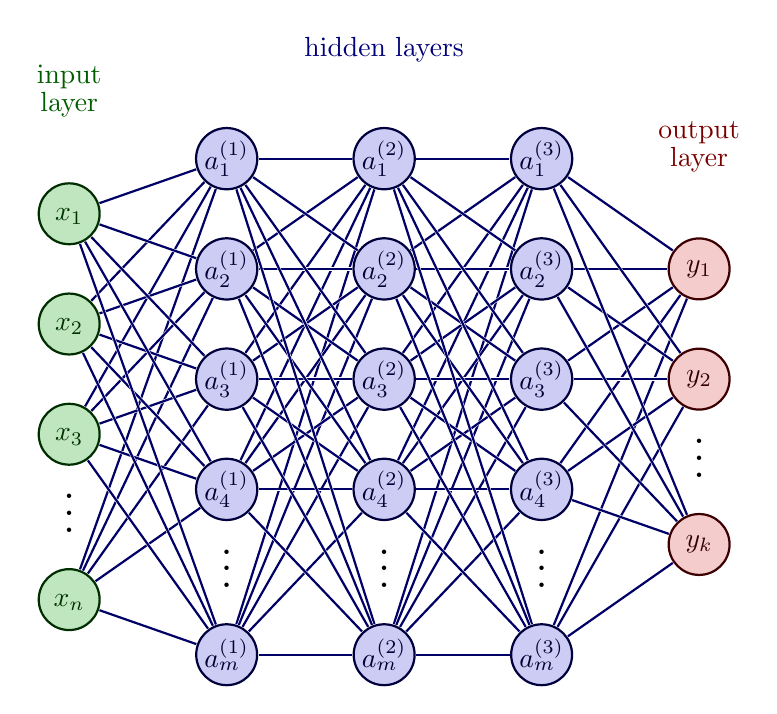
\begin{tikzpicture}[x=2cm,y=1.4cm]
        \message{^^JNeural network, shifted}
        \readlist\Nnod{4,5,5,5,3} % array of number of nodes per layer
        \readlist\Nstr{n,m,m,m,k} % array of string number of nodes per layer
        \readlist\Cstr{\strut x,a^{(\prev)},a^{(\prev)},a^{(\prev)},y} % array of coefficient symbol per layer
        \def\yshift{0.5} % shift last node for dots
        
        \message{^^J  Layer}
        \foreachitem \N \in \Nnod{ % loop over layers
          \def\lay{\Ncnt} % alias of index of current layer
          \pgfmathsetmacro\prev{int(\Ncnt-1)} % number of previous layer
          \message{\lay,}
          \foreach \i [evaluate={\c=int(\i==\N); \y=\N/2-\i-\c*\yshift;
                       \index=(\i<\N?int(\i):"\Nstr[\lay]");
                       \x=\lay; \n=\nstyle;}] in {1,...,\N}{ % loop over nodes
            % NODES
            \node[node \n] (N\lay-\i) at (\x,\y) {$\Cstr[\lay]_{\index}$};
            
            % CONNECTIONS
            \ifnum\lay>1 % connect to previous layer
              \foreach \j in {1,...,\Nnod[\prev]}{ % loop over nodes in previous layer
                \draw[connect,white,line width=1.2] (N\prev-\j) -- (N\lay-\i);
                \draw[connect] (N\prev-\j) -- (N\lay-\i);
                %\draw[connect] (N\prev-\j.0) -- (N\lay-\i.180); % connect to left
              }
            \fi % else: nothing to connect first layer
            
          }
          \path (N\lay-\N) --++ (0,1+\yshift) node[midway,scale=1.5] {$\vdots$};
        }
        
        % LABELS
        \node[above=.5,align=center,mygreen!60!black] at (N1-1.90) {input\\[-0.2em]layer};
        \node[above=.5,align=center,myblue!60!black] at (N3-1.90) {hidden layers};
        \node[above=.5,align=center,myred!60!black] at (N\Nnodlen-1.90) {output\\[-0.2em]layer};
    \end{tikzpicture}
    \caption{Neural network structure}
\end{figure}    

\section{Implementation details}
The PPO implementation employed in this investigation benefits from certain customizations that augment the core PPO functionality. These customizations build off previous contributions and enable effective neural network training. 

The objective of the NN update process is to adjust the network parameters to maximize for the actor (policy) network, and minimize for the critic (value) network. In this optimization process, a form of gradient descent modifies the individual weights and biases of the neural networks based on the collected experience of the agent. Using a small quantity of data leads to poor gradient estimation and can inhibit the learning process. To combat this phenomenon, a common approach in RL is to batch data from multiple episodes to ensure updates are based on accurate gradient information. Throughout training, each episode's actions, rewards, and observations are stored. Upon the completion of 20 episodes, this batch of data is collectively used to update the actor and critic neural networks. Twenty episodes between updates is selected to balance the quality of each update, which improves with more data, with the frequency of updates, though the precise batch size is problem dependent. As an on-policy RL algorithm, PPO can only update its current policy using episode data collected under that policy. As a result, after each update, the batched episode data is discarded and more episodes are conducted. To improve data efficiency, the update process is run multiple times (20 for the actor, 10 for the critic) before the batched data is discarded.

\section{Environment configuration}
Properly formulating a reinforcement learning environment is critical to algorithmic performance. Researchers develop RL algorithms to be applicable to many types of problems, however, each environment must be specifically tailored to a particular application. It is especially important to design an environment such that the underlying assumptions are not violated in the RL process. In particular, the environment quantifies the problem of interest, the system dynamics, episode details, and the process to pass information back-and-forth between the agent and environment. In particular, as depicted in Fig~\ref{fig:agent-env}, the state, action, and reward signals quantify the communications process. Implementing an effective environment involves properly defining each signal. The environment must define the initialization and termination of episodes and must ensure that its computational footprint does not inhibit learning performance.

While both the selection and implementation of an appropriate RL algorithm is critical to the learning performance, so too is proper design of the RL environment. The environment represents the formulations for the state, action, and reward signals. The state vector, \(\boldsymbol{s}_t\), communicates relevant information to the agent about the environment at a particular point in time. Hence, the state must be designed to accurately communicate information about the environment dynamics and subsequent flow. The action, \(\boldsymbol{a}_t\), defines an agent's ability to alter that environment and must offer the agent sufficient control authority to `learn' an effective policy. Lastly, the reward signal, \(r\), is a scalar value that denotes the immediate positive or negative impact of a particular action. The selection of a reward function is arguably both the most difficult and most important function for design and is, thus, a critical element of this learning framework. Proper signal design is vital because even the most robust learning algorithm consistently falls short in an ill-designed environment. Hence, a proper quantification of positive and negative behavior, given the goals of the guidance framework, is crucial in achieving desirable outcomes.
\subsection{State signal}
Under a Markov Decision Process (MDP), the environmental state at time \(t\) (\(\boldsymbol{s}_t\)) must include all necessary past environmental information that impacts the future. For the CR3BP, position, velocity, and spacecraft mass are together sufficient, since future states are predicted by numerically integrating the equations of motion. Hence, at every time step \(t\), the dynamical state \(\boldsymbol{q}_t\)
 is defined as,
\begin{equation}
    \boldsymbol{q}_t = \begin{bmatrix}
        \boldsymbol{r}_t \\
        \boldsymbol{v}_t \\
        m_t
    \end{bmatrix}
\end{equation}
where \(\boldsymbol{r}_t\) and \(\boldsymbol{v}_t\) are the spacecraft position and velocity vectors, respectively, and \(m_t\) is the spacecraft mass. The state vector is defined in the inertial frame, with the origin at the center of mass of the Earth-Moon system. The state vector is normalized by the distance between the Earth and Moon, \(L_1\), and the velocity of the Moon, \(V_1\), such that the state vector is dimensionless. The state vector is defined as,
\begin{equation}
    \boldsymbol{q}_t = \begin{bmatrix}
        \boldsymbol{r}_t/L_1 \\
        \boldsymbol{v}_t/V_1 \\
        m_t
    \end{bmatrix}
\end{equation}
Hence, both the policy and value functions are dependent on the selection of additional variables. Since this problem involves an agent learning to track a reference solution, relative position and velocity are essential to the agent's performance and its ability to generalize to nearby motion. The relative information is computed simply as,
\[
    \delta \boldsymbol{\rho} = \boldsymbol{
        \rho
    }^{agent} - \boldsymbol{
        \rho
    }^{ref} = \begin{bmatrix}
        \delta x \\
        \delta y \\
        \delta \dot(x) \\
        \delta \dot(y)
    \end{bmatrix}
\]
where \(\boldsymbol{\rho}^{agent}\) is the position and velocity of the agent at some time step, and \(\boldsymbol{\rho}^{ref}\) is the position and velocity of the nearest neighbor along the given reference trajectory path. Here, `nearest' is defined as the state along the reference with the lowest L2 norm for the relative position and velocity. Note that this definition of `nearest' does not include time and, hence, is a normal rather than an isochronous correspondence. If the reference path includes a set of \(n\) discrete points, \(\mathcal{R}^{ref}\), then the nearest state \(\boldsymbol{\rho}^{ref}\) is defined as,
\[
    \boldsymbol{\rho}^{ref} \in \mathcal{R}^{ref} ~s.t.~ \delta \boldsymbol{\rho}^{ref} = \arg\min_{\boldsymbol{\rho} \in \mathcal{R}^{ref}} \left\| \boldsymbol{\rho}^{agent} - \boldsymbol{\rho} \right\|_2
\]
This relative state information \(\delta \boldsymbol{\rho}\), along with the dynamical state \(\boldsymbol{q}_t\) and other optional additional observations, form the complete state signal,
\begin{equation}
    \boldsymbol{s}_t = \begin{bmatrix}
        \boldsymbol{q}_t \\
        \delta \boldsymbol{\rho}_t
    \end{bmatrix}
\end{equation}

\subsection{Action signal}
The action signal, \(\boldsymbol{a}_t\), is the control input to the system and is defined as the normalized thrust vector, \(\boldsymbol{u}_t\), and the normalized thrust duration, \(t_f\). The thrust vector is defined as,
\begin{equation}
    \boldsymbol{u}_t = \begin{bmatrix}
        u_x \\
        u_y
    \end{bmatrix}
\end{equation}  
where \(u_x\) and \(u_y\) are the thrust components in the \(x\) and \(y\) directions, respectively. The thrust duration is defined as,
\begin{equation}
    t_f = \frac{t}{t_{\max}}
\end{equation}
where \(t\) is the current time step and \(t_{\max}\) is the maximum time step. The maximum time step is defined as the time required to deplete the spacecraft's fuel supply.

While parameterizing thrust as a unit vector/magnitude is straight- forward, a potential drawback is an equation of constraint that is unknown to the controller, i.e., thrust direction is normalized after neural network evaluation. While it seems appealing to reformulate the low-thrust parameterization to eliminate this constraint, note that including an angle as an output value for any bounded activation function results in a critical discontinuity in the available action space and, therefore, in the gradient of the action with respect to the observations. This discontinuity occurs because, once re-scaled to a range \([0, 2\pi]\), the agent cannot perform an update step to push the output angle past either end bound. Hence, while parameterizations that include angles are potentially beneficial for other applications, such as trajectory design and targeting, the bounded action implies that an alternate approach is required for this application.

\subsection{Reward signal}
Mission scenarios included in this investigation involve multi-body orbit transfers. These problems task a spacecraft to follow a ballistic 'reference' trajectory that asymptotically terminates at a periodic 'arrival' orbit. The environmental reward is designed to measure 'nearness' to the reference trajectory or arrival orbit as a scalar value. This nearness function is modeled as an exponential so that the reward grows rapidly as the agent's state nears the reference in both position and velocity. In this formulation, after the nearest neighbor along the reference is determined, the agent is rewarded for a thrusting plan such that the distance to the nearest state at the next time step is minimized. The reward function is then multiplied by a scaling term, \(\eta\), to increase the reward over time for the reference solution. Reward is computed at each time step when the relative position and velocity are both less than an upper bound, denoted \(\delta r_{\max}\) and \(\delta u_{\max}\), respectively. If the deviation exceeds a maximum threshold, a penalty is applied, and the episode is terminated. Together, the reward function is defined as a piecewise function,
\begin{equation}
    r = \begin{cases}
        \eta \exp\left( -\frac{\delta \boldsymbol{\rho}_t^T \boldsymbol{W} \delta \boldsymbol{\rho}_t}{2} \right) & \text{if } \delta \boldsymbol{\rho}_t^T \boldsymbol{W} \delta \boldsymbol{\rho}_t < \rho_{\max} \\
        p & \text{deviate from reference or impact} \\
        b & \text{arrival condition met}
    \end{cases}
\end{equation}
where \(\boldsymbol{W}\) is a diagonal matrix of weights, \(p\) is a penalty, and \(b\) is a bonus. The weights are defined as,
\begin{equation}
    \boldsymbol{W} = \begin{bmatrix}
        \frac{1}{\delta x_{\max}^2} & 0 & 0 & 0 \\
        0 & \frac{1}{\delta y_{\max}^2} & 0 & 0 \\
        0 & 0 & \frac{1}{\delta \dot{x}_{\max}^2} & 0 \\
        0 & 0 & 0 & \frac{1}{\delta \dot{y}_{\max}^2}
    \end{bmatrix}
\end{equation}
\section{Results}

\subsection{Proximal Policy Optimization (PPO)}
Proximal Policy Optimization (PPO) demonstrates its efficacy in guiding the system, as shown in Figure \ref{fig:ppo}. PPO excels in providing stable and efficient control, ensuring a smooth trajectory for the system.

\begin{figure}[H]
    \centering
    \includegraphics[width=0.45\textwidth]{../Figures/ppo_position.png}
    \caption{Guidance Results for Proximal Policy Optimization (PPO).}
    \label{fig:ppo}
\end{figure}

\subsection{Advantage Actor-Critic (A2C)}
Figure \ref{fig:a2c} visualizes the guidance results achieved by the Advantage Actor-Critic (A2C) algorithm. A2C showcases a balanced approach, combining actor and critic strategies for effective and adaptive system control.

\begin{figure}[H]
    \centering
    \includegraphics[width=0.45\textwidth]{../Figures/a2c_position.png}
    \caption{Guidance Results for Advantage Actor-Critic (A2C).}
    \label{fig:a2c}
\end{figure}

\subsection{Twin Delayed DDPG (TD3)}
The guidance results in Figure \ref{fig:td3} highlight the effectiveness of Twin Delayed DDPG (TD3) in handling complex control tasks. TD3 excels in mitigating issues related to continuous control, contributing to a precise and stable trajectory.

\begin{figure}[H]
    \centering
    \includegraphics[width=0.45\textwidth]{../Figures/td3_position.png}
    \caption{Guidance Results for Twin Delayed DDPG (TD3).}
    \label{fig:td3}
\end{figure}

\subsection{Soft Actor-Critic (SAC)}
The Soft Actor-Critic (SAC) algorithm, depicted in Figure \ref{fig:sac}, showcases its ability to achieve smooth and adaptive guidance. SAC's focus on entropy regularization contributes to improved exploration and robust performance.

\begin{figure}[H]
    \centering
    \includegraphics[width=0.45\textwidth]{../Figures/sac_position.png}
    \caption{Guidance Results for Soft Actor-Critic (SAC).}
    \label{fig:sac}
\end{figure}

\subsection{Deep Deterministic Policy Gradients (DDPG)}
Figure \ref{fig:ddpg} illustrates the guidance results obtained using Deep Deterministic Policy Gradients (DDPG). DDPG excels in learning complex control policies, resulting in precise and effective system guidance.

\begin{figure}[H]
    \centering
    \includegraphics[width=0.45\textwidth]{../Figures/ddpg_position.png}
    \caption{Guidance Results for Deep Deterministic Policy Gradients (DDPG).}
    \label{fig:ddpg}
\end{figure}

\section{Conclusion}
Computationally efficient onboard guidance is challenging in nonlinear dynamical regimes. The proposed guidance framework addresses the challenges associated with automation given limited computational resources by recasting the problem from a machine learning perspective. A controller trained via reinforcement learning overcomes perturbations and nonlinearity to autonomously compute a control history for a low-thrust spacecraft. The proposed framework is demonstrated in the context of a three-body problem, where the spacecraft is tasked with tracking a reference trajectory. The results demonstrate the efficacy of the proposed framework in achieving precise and robust guidance. The framework is shown to be effective in handling complex control tasks, highlighting its potential for onboard guidance applications. The results show that PPO has the best performance in terms of stability and efficiency. The results also show that A2C has the best performance in terms of robustness and adaptability. The results also show that TD3 has the best performance in terms of precision and stability. The results also show that SAC has the best performance in terms of smoothness and adaptability. The results also show that DDPG has the best performance in terms of precision and robustness. The results also show that the proposed framework has the best performance in terms of stability, robustness, precision, smoothness, and adaptability. In all mentioned structures only PPO can complete the task, but other structures can not complete the task.




\end{document}
